\documentclass{book}
\usepackage{mathpackages}
\usepackage{mathcommands}
%====uncomment this AND at the end and when I want an index======================= 
\makeindex 
%======================
\begin{document}

\title{Mathematical Formalizations: A brief study guide}
 \author{\includegraphics[width=0.9\textwidth]{Screenshot-1}\\ Joshua Bowles\\ \date{\today}}
         
\maketitle

%=================uncomment this when I want list of figures and tables
\tableofcontents 
\listoffigures 
\listoftables 
  
%==========
\chapter*{Preface}
\begin{quote}
     \textsl{Immature poets imitate; mature poets steal; bad poets deface what they take, and good poets make it into something better, or at least something different}.\\ --T.S. Eliot
\end{quote}


I would imagine the quote from Eliot could apply also to world of mathematics; one might addend it with the line ``and genius creates directly from nature.'' I am far from a mature mathematician, and hope one day to be a good one; at least in terms of my respective field of application and theory of mathematical formaliztions to the study of natural language linguistics. If the quote above were truely accurate here then I would be doing more imitating then stealing\ldots, but the truth is that I do more stealing than anything.

This book is intended as a study guide for myself; if you are reading it then I have made it public for whatever reason. \textcolor{red}{\textbf{Please do not cite this reference guide}}. I have taken liberally from multiple sources and have not been too cautious in making sure that I have not plagiarized. The reason for this is becuase I want to make sure the mathematics I present here is credible: proofs, examples, theorems, and so on. I have modified many examples and such, but only when I was sure of the outcome; if there was every any question on my part I simply copied freely in order to ensure that this personal study guide was true to the facts. 

The following sources have both inspired and guided me, and represent sources that I have either borrowed from, or flatly taken taken material out of (without permission by the way): \cite{gustfriskalgebra}, \cite{mathbook}, \cite{pmw:1990}, \cite{kleene:1967}, and \ldots. Of particular note is \cite{silvthomp}, originally written in 1910, and commendable for its Prologue which bears quoting in length.

\begin{quotation}
    Considering how many fools can calculate, it is surprising tha tit should be thought either a difficult or a tedious task for any other fool to learn how to master the same tricks.

Some calculus-tricks are quite easy. Some are enormously difficult. The fools who write the text-books of advanced mathematics---and they are mostly clever fools---seldom take the trouble to show you how easy the calculations are. On the contrary, the see to desire to impress you with their tremendous cleverness by going about it in the msot difficult way.

Being myself a remarkably stupid fellow, I have had to unteach myself the difficulties, and now beg to present to my fellow fools the parts that are not hard. \ldots What one fool can do, another can.
\end{quotation}

\chapter*{Prologue}
 The quotation by Silvanus Thompson was written in time when a calculator (or better yet, a calculat-er) was an individual hired to plug variables into algorithms and perform other kinds of calculations. One could possibly see on a day to day basis, in Silvanus' day, that one did not need to be exceptionally bright in order to perform calculations. Today, we have sophisticated tools like scientitifc calculators, computational software, and computers to do the calculating for us. It is easy to be mistified by the process of brute calculation and from the depths of this mistification even easier to be lead into beleiving that calculation is an entirely difficult acitivty. Silvanus' humor, self-deprecation, and ease of exposition should be a model in both teaching and learning math. His all-around attitude is far too uncommon in a world that more resembles priests of some high-order who have secret knowledge of symbols and stand guard at the gates, waiting to dispel the weakest of underlings who dares try to join thier society than a mysterious world full of puzzles and beauty waiting to be explored by active young minds with rigorous tools developed thorugh the amazing history of human consciousness. One rarely hears about how mathematical developments rival the beauty and creativity of other human achievments in art, literature, music, and architecture. Silvanus' distinct attitude towards mathematics is conducive to the latter musings, and I hope to emulate his strength of character and appreciation for formalization.

I prefer to think of math like I often tell my daughters: doing math is like digging a ditch. It seems simple when you think about what needs to be done; that is, combining like properties or solving variables or employing various binary combinations on vaalues, \textsl{et cetera}. What is hard is the actual work involved -- and the patience, discipline, and strength building that is necessitated by such work. 

%==================
%===========Comment out for Book==================

% \documentclass{book} \usepackage{mathpackages} \begin{document} 
%====================================

\chapter{Arithmetic}
In this chapter I sketch the basic materials of arithmetic. 
      \section{Percent}
Any percent\index{percent} can be transformed into a rational number fraction by dividing by 100, which also gives a decimal:
\[ 40\% = \frac{40}{100} = .4 \]
Multiplying decimal values by other numerical values will yield a percentage relation. For example,
\[ 30\% \text{ of } 350 = (350)\left(\frac{30}{100}\right) = (350)\left(\frac{3}{10}\right) = \frac{1,050}{10} = 105 \] 
or,
\[ 30\% \text{ of } 350 = .3\times350 = 105 \]

Increases (equation \ref{greater}) and decreases (equation \ref{less}) of percentages are handled by the following; assume that x and y are positive numbers and that $x < y$:
\begin{equation}\label{greater}
    y \text{ is }\left(\frac{y-x}{x} \right)(100) \text{ percent greater than } x
\end{equation}
\begin{equation}\label{less}
     x \text{ is }\left(\frac{y-x}{y} \right)(100) \text{ percent less than } y
\end{equation}
For example, an \textbf{increase} from 600 to 750 is found by dividing the difference of the increase (750 - 600 = 150) by the first or \textbf{smaller} of the two initial values, known as the \textsl{base}, or the denominator:
\[ \left(\frac{150}{600}\right)(100) = 25\%\]
Whereas a \textbf{decrease} from 500 to 400 is found by dividing the difference of the decrease (500 - 400 = 100) by the first or \textbf{larger} of the two initial values, also known as the \textsl{base}, or the denominator:
\[ \left(\frac{100}{500}\right)(100) = 20\%\]

      \section{Average and Arithmetic Mean}
\begin{align}
    \frac{x_1 + y_2 + z_3}{3} &= \text{average}\\
\frac{n_m}{m} &= \text{average}
\end{align}
\begin{example}
      \begin{equation}
   \begin{split}
\frac{5_1 + 8_2 + 8_3 + 14_4 + 15_5 + 10_6}{6} &= Average(x)\\
 \frac{60}{6} &= 10
   \end{split} 
      \end{equation}
\end{example}


   \subsection{Range}
Range is defined as the greatest measurement minus the least measurement, iff all numerical values are a discrete set. 
\begin{align}
    \textcolor{red}{5}, 8, 8, 14, \textcolor{red}{15}, 10 &= Range(x)\\
15 - 5 &= 10
\end{align}
Notice that it is a coincidence that the {\sl range} and the {\sl average} are the same value. Range by itself is not very useful, but has been used as the starting intuition for developing the \textsl{standard deviation}.

   %\subsection{Standard deviation}

   %\subsection{Frequency distribution}



%======================
\chapter{Basic Geometry}
      \section{Area, Perimeter, Volume}
   \subsection{Area}
Triangle:
\begin{equation}
    A = \frac{bh}{2} \qquad \text{\scriptsize b = base, h = height}
\end{equation}
Square:
\begin{equation}
    A = l^2 \qquad \text{\scriptsize l = length}
\end{equation}
Rectangle:
\begin{equation}
    A = bh \qquad \text{\scriptsize b = base, b = height}
\end{equation}
Regular Polygons:
Add this later\ldots\\
Circle:
\begin{equation}
    A = \pi r^2 \qquad \text{\scriptsize r = radius}
\end{equation}

   \subsection{Perimeter}\label{perimeter}
Triangle:
\begin{equation}
    P = l_a + l_b + l_c \qquad \text{\scriptsize l = length}
\end{equation}
Square:
\begin{equation}
    P = 4l \qquad \text{\scriptsize l = length}
\end{equation}
Rectangle:\footnote{Perimeter for a rectangle can also be defined equivalently as $P = 2(l + w)$, where l = length and w = width, or as $P = 2(side A + side B)$}
\begin{equation}
    P = 2(b + h) \qquad \text{\scriptsize b = base, h = height}
\end{equation}
Regular Polygons:
\begin{equation}
    P = nl \qquad \text{\scriptsize l = length, n = number of sides}
\end{equation}
Circle (\textsl{circumfrence}):
\begin{equation}
    C = 2 * \pi * r \qquad \text{\scriptsize C = circumfrence, r = radius}
\end{equation}

   \subsection{Volume}
Cone or Pyramid:
\begin{equation}
    V = \frac{1}{3}(bh) \qquad \text{\scriptsize b = base, h = height}
\end{equation}
Cube:
\begin{equation}
    V = l^3 \qquad \text{\scriptsize l = length}
\end{equation}
Rectangular prism:
\begin{equation}
    V = bwh \qquad \text{\scriptsize b = base, w = width, h = height}
\end{equation}
Sphere:
\begin{equation}
    V = \frac{4}{3}\pi r^3 \qquad \text{\scriptsize r = radius}
\end{equation}
Cylinder:
\begin{equation}
    V = A_{base} * h \qquad \text{\scriptsize $A_{base}$ = area of base, h = height}
\end{equation}

      \section{The Circle}
For a circle, the \textsl{radius} is measured from the midpoint to an edge, \textsl{diameter} is any line that meets two edges and passes through the center point; any line that touches two edges but does not pass through the mid point is called a \textsl{chord}.

The ration of circumference to diameter of a circle is 
\begin{equation}
    \frac{c}{d}\pi
\end{equation}
Circumference, given above in \ref{perimeter}, is repeated here:
\begin{equation}
    c = 2\pi r
\end{equation}

      \section{Pythagorean theorem}\index{Pythagorean theorem}
\begin{equation}
    a^2 + b^2 = c^2
\end{equation}
      \section{Polygons}
\subsection{Sums for interior polygon angles}
The sum of the interior angles for any $n$-sided polygon\index{polygon} is:
\begin{equation}
    (n - 2)(180^\circ) 
\end{equation}
For example, where $n$ equals any real value for triangle, quadrilateral, pentagon, hexagon, etc.:
\begin{equation}
 \begin{split}
(3-2)(180^\circ)& = 180^\circ\\
(4-2)(180^\circ)& = 360^\circ\\
(5-2)(180^\circ)& = 540^\circ\\
(6-2)(180^\circ)& = 720^\circ\\
(7-2)(180^\circ)& = 900^\circ\\
(8-2)(180^\circ)& = 1080^\circ\\
(9-2)(180^\circ)& = 1260^\circ\\
(10-2)(180^\circ)& = 1440^\circ
\end{split}   
\end{equation}
Notice the the difference between $n \pm1$ side for the sum of interior angles is $180^\circ$, that is, adding or subtracting one side to a polygon is equivalent to increasing or decreasing the sum of the interior angles by $180^\circ$. We can state this as a co-variation, where the number of sides varies directly\index{direct variation of polygon sides} with the value 180; where $k = 180$ and is the constant:
\begin{equation}
    y =kx \qquad \text{or} \qquad \frac{y}{x} =k
\end{equation}
The following show the direct variation\index{direct variation of polygon angles} of the sum of interior angles for polygons\index{polygon}; first a quadrilateral, then a pentagon:
\begin{equation}
    360 =(180)(4-2) \qquad \text{or} \qquad \frac{360}{4-2} =180
\end{equation}
and,
\begin{equation}
    540 =(180)(5-2) \qquad  \text{or} \qquad \frac{540}{5-2} =180
\end{equation}
An interesting thing that falls out of this series for polygons is the definition of line.\footnote{According to the polygonal series and the direct variation defined above, a line, with 0 angles, ends up being $-360^\circ$. Another way is to start with a line as defined as having 0 degree: by this path we have to give a line 2 sides so that $0 \times 180 = 0$.} Defining a line by this method could be used as a proof for why a line is not a polygon; I leave this up to imagination.

   \subsection{Area and Perimeter for Polygons}
The \textsl{perimeter} of a polygon is the sum of the lengths of its sides. The \textsl{area} of a polygon is the measure of enclosed region.

   \subsubsection{Triangles}
\begin{maxim}
No triangle can have a longest side that is greater than the sum to the two shortest sides.
\end{maxim}
\begin{example}
    If triangle $\bigtriangleup$ABC has $A = 4$, $B = 7$, then $C \neq 12$. That is, $4 + 7 =11$, and since no side of a triangle can be greater than the sum of two other sides, C cannot be greater than $11$. In other words, take the longest side of $\Delta$ABC, the sum of the other sides cannot be greater.
\end{example}
\begin{definition}\textsc{Equilateral Triangle}\\
Has all three sides equal
\end{definition}
\begin{example}
    For equilateral $\bigtriangleup$ABC, all angles must equal $60^\circ$. If any angle is more or less than 60, then $\bigtriangleup$ABC $\neq 180$.
\end{example}

\begin{definition}\textsc{Isosceles Triangle}\\
Has two sides of equal length. 
\end{definition}
\begin{example}
    For isosceles $\bigtriangleup$ABC, angle ABC and angle BCA = $50^\circ$, then
\begin{align*}
    50 + 50 + x &= 180\\
   100 + x &= 180\\
   x &= 80
\end{align*}
\end{example}

\begin{definition}\textsc{Right Triangle}\\
Has one interior angle that equals $90^\circ$. For right $\bigtriangleup$DEF, say DF is hypotenuse (side oposite of the right angle), then Pythogorean theorem says that $(DF)^2 = (DE)^2 + (EF)^2$
\end{definition}
\begin{example}
    For right $\bigtriangleup$DEF, DE = 5, DF = 8 and is the hypotenuse, and EF = x, then
\begin{align*}
    8^2 &= 5^2 + x^2\\
   64 &= 25 + x^2\\
   39 &= x^2
\end{align*}
\end{example}

%===========Comment out for Book=========
% \end{document}
%====================

%==================================================
%===========Comment out for Book==================
\documentclass{book}  \usepackage{mathpackages,mathcommands}  \begin{document} 
%====================================

\chapter{Elementary Algebra: Equations and Formulas}
      \section{The Quadratic Equation}
\begin{equation}
    ax^2 + bx + c = 0
\end{equation}
There are two main ways of solving: by factoring or by the quadratic formula.
	 
	 \subsection{Factoring quadratics}
The following quadratic equation\index{quadratic equation} is solved by factoring and setting the factors to zero.
\begin{equation}
    2x^2 -x -6 = 0
\end{equation}

         \begin{center}
      \begin{tabular}{|l|l|l|}
\hline
Factor & Set to 0; solve & Set to 0; solve\\
\hline\hline
$(2x + 3)(x - 2)=0$ & $2x + 3 = 0$ & $x -2 = 0$\\
{}                & $ 2x + 3 = 0 $ & \textcolor{magenta}{$ x = 2$}\\
{}                & $2x = -3$ & {}\\
{} & \textcolor{magenta}{$x = -\dfrac{2}{3}$} & {}\\
\hline
         \end{tabular}
            \end{center}
Other factorable quadratics are:
\begin{equation}
    x^2 +8x +15 = 0
\end{equation}

         \begin{center}
      \begin{tabular}{|l|l|l|}
\hline
Factor & Set to 0; solve & Set to 0; solve\\
\hline\hline
$(x + 3)(x + 5)=0$ & $x + 3 = 0$ & $x +5 = 0$\\
{}               & \textcolor{magenta}{$x = -3$} & \textcolor{magenta}{$ x = -5$}\\
\hline
         \end{tabular}
            \end{center}

\begin{equation}
    4x^2 -9x [\pm 0] = 0
\end{equation}
Notice that this quadratic's third term can be plus or minus zero, and also that it can be factored as the difference of two squares $x^2$ and $3^2$.
         \begin{center}
      \begin{tabular}{|l|l|l|}
\hline
Factor & Set to 0; solve & Set to 0; solve\\
\hline\hline
$(2x + 3)(2x - 3)=0$ & $2x + 3 = 0$ & $2x -3 = 0$\\
{}                   & $2x = 3$     & $2x = -3$\\ 
{}               & \textcolor{magenta}{$x = \dfrac{3}{2}$} & \textcolor{magenta}{$x = -\dfrac{3}{2}$}\\
\hline
         \end{tabular}
            \end{center}
   
	 \subsection{Quadratic Formula}
A quadratic expression $ax^2 +bx +c = 0$ can also be solved by randomly assigning numerical values to the variables in the following quadratic formula\index{quadratic formula}; although true random assigment is not possible, as I make clear below.

\begin{equation}
    x = \dfrac{-b \pm \sqrt{b^2 - 4ac}}{2a}
\end{equation}

For example, the equation \textcolor{magenta}{$2x^2 -x -6 =0$}; where \textcolor{red}{a = 2}, \textcolor{blue}{b = -1}, and \textcolor{green}{c = -6} yields the following:
\begin{equation}
    x = \frac{-(\textcolor{blue}{-1}) \pm \sqrt{(\textcolor{blue}{-1})^2 - 4(\textcolor{red}{2})(\textcolor{red}{-6}})}{2(\textcolor{green}{2})}
= \frac{1 \pm \sqrt{49}}{4}
= \frac{1 \pm 7}{4}
\end{equation}\label{zero}

The $\pm$ solutions are then \textcolor{magenta}{$x = \frac{1+7}{4} = 2$} and \textcolor{magenta}{$x = \frac{1-7}{4} = -\frac{3}{2}$}. 
As usual with fractionals, apparent solutions that produce a zero denominator are undefined and incorrect. For example, $a \neq 0$. If so, the denominator is 2(0) = 0, giving $\frac{X}{0}$, which is undefined. 

Lastly, most quadratics have at most two real solutions, but some only have one. For example, the following equation has one solution, \textcolor{blue}{x = -2} 
\begin{equation}
    x^2 + 4x + 4 = 0
\end{equation}
\[\textcolor{blue}{-2}^2 + 4(\textcolor{blue}{-2}) + 4 = 0 \]
\[ 4 + -8 + 4 = 0 \] 
\[-4 + 4 = 0
\]

Some quadratic\index{quadratic} problems have no solution.
 \begin{equation}
     x^2 + x + 5 = 0
 \end{equation}\label{nosolution}
A simple way to find out how many solutions to a quadratic\index{solutions to a quadratic} exist is to find the value of the \textcolor{magenta}{$b^2 - 4ac$} portion of the formula; this is called the discriminant\index{discriminant} and is symbolized by $\Delta$.
     
\begin{table}\caption[Solutions to Quadratic]{Discriminant value for number of solutions to quadratic} 
      \begin{center}
   \begin{tabular}{|r|l|}
\hline
If $\Delta > 0$ & there are two unique real solutions\\
If $\Delta = 0$ & there is one unique real solution\\
If $\Delta < 0$ & there are two unique, conjugate\\
{} & imaginary solutions\\
If $\Delta$ is perfect square & two solutions are rational,\\
{} & otherwise irrational conjugates\\
\hline
   \end{tabular}
      \end{center}
\end{table}
\vspace{.5in}
  
      \section{Two maxims for inequalities}
Inequalities\index{inequality} work like most equations. The two maxims below give the rules for direction of inequality when a combinatory operation is done on both sides. The maxims can also be defined in a different way by the the corollary that follows them.
\begin{maxim}\textbf{Additive Maxim}\\
When the same constant is added to (or subtracted from) both sides of the inequality, the direction of inequality is preserved. And, the new inequality is equivalent to the old inequality.
\end{maxim}
\begin{maxim}\textbf{Multiplicative Maxim}\\
When the same constant is multiplied to (or divided from) both sides of the inequality, \textsl{the direction of inequality is preserved iff the constant is positive, but reversed if the constant is negative}. In both cases, the new inequality is equivalent to the old inequality.
\end{maxim}

\newtheorem*{corollmaxim}{Corollary to Inequality Maxims}
\begin{corollmaxim}
An inequality can change direction iff both sides of the inequality are multiplied (or divided) by the same negative constant. 
\end{corollmaxim}

      \section{Sequences}
\begin{definition}
A \textbf{sequence}\index{sequence} can be defined as a \textsc{function} whose \textcolor{red}{domain}\index{domain} is the set of real numbers.    
\end{definition}
Sequences are typically given as lists or series. For example, the function $f(n) =2n-1$ will output a range over the real numbers. Notice that the function defines a sequence of the real numbers as a kind of subsequence that the function\index{function} is supposed to use as the domain/input -- this is why the definition explicitly mentions the set of real of numbers as the domain. But the presuppostion is stronger than simply assigning by definition the domain\index{domain} for the function; it in fact assumes that where one begins the subsequence is arbitrary. In other words, in the following example, I arbitrarily decided to start the subsequence at 0; also notice that it is possible to have my subsequence running at non-regular (perhaps even random) intervals such as $1, \frac{1}{2}, \frac{2}{3}, \sqrt{3},\ldots$ . 
\begin{align*}
    \textcolor{blue}{f(n)} &= \textcolor{blue}{2n -1}\\
\textcolor{blue}{f(n)} &= [\textcolor{blue}{2(1) -1} =1], [\textcolor{blue}{2(2) -1} =3], [\textcolor{blue}{2(3) -1} =5], [\textcolor{blue}{2(4) -1} =7], \ldots \\
&= 1, 3, 5, 7, 9, 11,\ldots\\
\textcolor{blue}{f(n)} &= [\textcolor{blue}{2(1) -1} =1], [\textcolor{blue}{2(\frac{1}{2}) -1} =0], [\textcolor{blue}{2(\frac{2}{3}) -1} =.\bar{3}], [\textcolor{blue}{2(\sqrt{3}) -1} =2.464], \ldots\\
&= 1, 0, .\bar{3}, 2.464,\ldots 
\end{align*}

	 \subsubsection{A Recursive Definition}
Any sequence can be given a recursive definition\index{recursive definition} by giving the first term and a rule that shows how to obtain further terms; i.e., how to get the $(n + 1)th$ term from the $n$th term. Here is a general formulation followed by a specific example.
\begin{align}
    a_1 &= x \; \; \text{\textcolor{red}{($n$th term)}} \nonumber  \\ 
a_n+1 &= y \; \; \text{\textcolor{red}{(recursive rule)}} 
\end{align}
      \begin{align}
a_1 &= 5 \; \; \text{\textcolor{red}{($n$th term)}} \nonumber \\ 
a_n+1 &= 3a_n -2 \; \; \text{\textcolor{red}{(recursive rule)}} \nonumber \\
\text{therefore,} \nonumber \\
a_1 &= \textcolor{blue}{5} \nonumber \\ 
a_2 &= 3(a_1 (= \textcolor{blue}{5})) - 2 = \textcolor{blue}{13} \nonumber \\
a_3 &= 3(a_2 (= \textcolor{blue}{13})) -2 = \textcolor{blue}{37} \nonumber \\
a_4 &= 3(a_3 (= \textcolor{blue}{37})) -2 = \textcolor{blue}{109} \nonumber \\
a_5 &= 3(a_4 (= \textcolor{blue}{109})) -2 = \textcolor{blue}{325}
      \end{align}
Here we can see the details in the popular generative linguistic\index{generative linguistics} definition of recursiveness\index{recursiveness} that points out that a certain kind of recursion (tail-recursion) provides input\index{input} for the new function from the output\index{output} of the previous function\index{function}. For example, the new function $a_2$ is given the input $a_1 = 5$ (where 5 is the output of the function $a_1$) according to the recursive rule\index{recursive rule}.

      \section{Arithmetic and Geometric Sequences}\label{a-seq}
\subsection{A-Sequence} An \textbf{arithmetic sequence}\index{arithmetic sequence} is in the form
\begin{equation}\label{aseq}
    (a)_1,\quad (a +d)_2, \quad (a +2d)_3, \quad (a+3d)_4, \ldots, (a+ (n-1)d)_n, \ldots
\end{equation}
where \textcolor{red}{$a$ = first term} of the sequence, \textcolor{blue}{$a +(n-1)d$ = $n$th term} of the sequence, \textcolor{teal}{$n$ = number of terms}, and \textcolor{orange}{$d$ = common difference} of the terms. I have subscripted the seuqential terms in order to point out the fact that the first term $a_1$ has an addend of 0, the second term is $d$, or 1, the third term $2d$, or 2, the fourth term is $3d$ and so on. This is why the $n$th term is $n-1$. Some examples of adding sequences\index{adding sequences} follow.
\begin{example}
    Write the first 6 terms and the 10th term of an arithmetic sequence with a first term of 7 and a common difference of 5. 
\end{example}

\begin{solution}
    Since the first term is 7 and the common difference is 5, we can get the first 6 terms:\\
\indent \indent 7, 7 + 5, 7 + 2(5), 7 + 3(5), 7 + 4(5), 7 + 5(5)\\
or\\
\indent \indent 7, 12, 17, 22, 27, 32\\
Finding the 10th term requires substituting 10 for $n$ in the formula for arithmetic sequence in \ref{aseq}:
   \begin{align}
    n\text{th term} &= a + (n -1)d \nonumber\\
   21\text{st term} &= 7 + (10 -1)5\nonumber \\
   &= 7 + (9)5 = 52
   \end{align}
\end{solution}

Of course, if given the first term $a$ and the common difference $d$ one can just simply add terms until getting to the $n$th term. The next example shows how this method would become tedious.

\begin{example}
    Find the 98th term of an arithmetic sequence whose first three terms are 2, 6, 10.
\end{example}
\begin{solution}
    First step is to find common difference $d: 10 -6 =\textcolor{blue}{4}, 6 -2 =\textcolor{blue}{4}.\ d = \textcolor{blue}{4}$. Then we can substitute variables in formula \ref{aseq}: $a = 2, n = 98$. Now plug in the solution.
   \begin{align}
       n\text{th term} &= a + (n - 1)d \nonumber \\
      98\text{th term} &= 2 + (98 -1)4 \nonumber \\
&= 2 + (97)4 = 390
   \end{align}
Adding terms by 4 for 97 consequentive terms would be a waste of time, even on a calculator.
\end{solution}

\subsubsection{Arithmetic means}
These are numbers inserted between a first and last term to form a segment of an a-sequence. The method here is to assume a \textcolor{cyan}{last term $l$} as the $n$th term of the arithemtic sequence in \ref{aseq} 
\begin{equation}\label{a-mean}
    l = a + (n -1)d
\end{equation}
\begin{example}
    Insert three means between -3 and 12.
\end{example}
   \begin{solution}
    To insert three terms between the two we already have gives a total of 5 terms such that $n =5$. We are given the first and last terms: $a = 3, l = 12$. What we do not know is the common difference $d$:
      \begin{align}
    l &= a + (n -1)d\nonumber \\
12 &= -3 + (5 -1)d \nonumber \\
15 &= 4d \quad \text{\textcolor{red}{(Add 3 to both sides)}}\nonumber \\
\frac{15}{4} &= d \quad \text{\textcolor{red}{(Divide both sides by 4)}}
      \end{align}
Now with $d = \frac{15}{4}$ we plug in variables for finding the three middle terms which is really just part of the formula for arithmetic sequences in \ref{aseq} and can be represented as $(a +d)_2, \ (a +2d)_3, \ (a+3d)_4$, which is the sequence minus the first and $n$th (last) term.
      \begin{align}
          a + d &= -3 + \frac{15}{4} = \frac{3}{4} \nonumber \\
	 a + 2d &= -3 + 2\frac{15}{4} = -3 + \frac{30}{4}  = 4\frac{1}{2} \nonumber \\
	 a + 3d &= -3 + 3\frac{15}{4} = -3 + \frac{45}{4}  = 8\frac{1}{4} 
      \end{align}
The whole sequence, then, is \ \textcolor{purple}{-3, $\frac{3}{4}, 4\frac{1}{2}, 8\frac{1}{4}$, 12}
   \end{solution}
\subsubsection{Sum of first $n$ a-sequence terms}
The first $n$ terms of an arithmetical sequence\index{sum of first $n$} can also be calculated.
\begin{equation}\label{sum-of-first-n}
    S_n = \frac{n(a+l)}{2}
\end{equation}
where, as above,  \textcolor{red}{$a$ = first term} of the sequence, \textcolor{blue}{$a +(n-1)d$ = $n$th term} (or \textcolor{cyan}{$l = [a +(n-1)d]$ = last term}) of the sequence, and \textcolor{teal}{$n$ = number of terms}. 
\begin{example}
    Find the sum of the first 30 terms of the arithmetic sequence 5, 8, 11, \ldots .
\end{example}
\begin{solution}
    Plug-in the variables: $a =5, \ n = 30, \ d = 3, \ l = [5 + (30 -1)3] = 92$\\
and substitute into the formula from \ref{sum-of-first-n} to get
\begin{align}
    S_n &= \frac{n(a + l)}{2} \nonumber \\
S_{30} &= \frac{30(5 + 92)}{2} \nonumber \\
&= 15(97) = 1,455  
\end{align}

\end{solution}

\subsection{G-Sequence} 
A \textbf{geometric sequence}\index{geometric sequence} is in the form
\begin{equation}\label{gseq}
    (a)_1, \quad (ar)_2, \quad (ar^2)_3, \quad (ar^3)_4, \ldots, (ar^{n-1})_n, \ldots
\end{equation}
where \textcolor{red}{$a =$ first term} of the sequence, \textcolor{blue}{$ar^{n-1} = nth$ term} of sequence, and \textcolor{orange}{$r =$ common ratio}. Just as arithmetical sequences, I have numbered the terms by subscript to highlight the fact that the first term $a_1$ has no power, the second term $ar_2$ has power of 1, the third has power of 2, and so on. This is why the $n$th term power is $n-1$.
\begin{example}
    Write the first 6 terms and the 25th term of the geometric sequence whose first term = 3 and common ratio = 2.
\end{example}
   \begin{solution}
       Plugin the variables:\\
\indent \indent $3, \ 3(2), \ 3(2)^2, \ 3(2)^3, \ 3(2)^4, \ 3(2)^5$\\
or\\
\indent \indent 3, 6, 12, 24, 48, 96\\
For the 25th term simple computation is a waste of time. Instead, substitute 25 for $n$; as well as the other variables in the formula for the $n$th term that is at the end of the formula in \ref{gseq}.
      \begin{align}
          n\text{th term} &= ar^{n-1} \nonumber \\
	 25\text{th term} &= 3(2)^{25-1} \nonumber \\
	 3(2)^{24} &= 50,331,648
      \end{align}
   \end{solution}

      \subsubsection{Geometric means}
Geometric means are similar to arithmetical means.
\begin{example}
    Insert two geometric means between 4 and 256.
\end{example}

\begin{solution}
    Inserting two means within two terms give us a total of 4; $n = 4$. Plug-in the rest of the variables: first term $a =4$; last term is assumed to be the $n$th term. What we need is $r$:
\begin{align}
    ar^{n-1} &= l \nonumber \\
     4r^3 &= 256 \nonumber \\
    r^3 &= 64 \ \text{\textcolor{red}{(Divide both sides by 4)}} \nonumber \\
   r &= 4 \ \text{\textcolor{red}{(Find cube root on both sides)}}
\end{align}
Now that we have $r$, just plug-in variables for the second and third terms in the geometric sequence in \ref{gseq}.
 \begin{align}
     (ar)_2 &= 4 * 4 = 16 \nonumber \\
      (ar^2)_3 &= 4 * 4^2 = 4 * 16 = 64
 \end{align}
\end{solution}
The final sequence is 4, 16, 64, 256.

      \subsubsection{Sum of first $n$ g-sequence terms}
The sum of the first $n$ terms of a geometric sequence can be found by the following formula:
\begin{equation}\label{sum-first-n-g-seq}
    S_n = \frac{a - ar^n}{1 - r} \quad \textcolor{gray}{r \neq 1}
\end{equation}
The usual variables for sequences applies: where \textcolor{red}{$a$ = first term} of the sequence, \textcolor{blue}{$a +(n-1)d$ = $n$th term} (or \textcolor{cyan}{$l = [a +(n-1)d]$ = last term}) of the sequence, and \textcolor{teal}{$n$ = number of terms}.

   \subsection{Infinite Geometric Sequences}
Under certain conditions, we can find the sum of all the terms in an \textbf{infinite g-sequence}. To define this sum, consider the following g-sequence \textcolor{red}{$a, \ ar, \ ar^2, \dots$}
\begin{align*}
a &= S_1 \quad \text{\textcolor{gray}{The first partial sum of the sequence}}\\
a + ar &=  S_2  \quad \text{\textcolor{gray}{The second partial sum of the sequence}} \\
a + ar + ar^2 + \cdots + ar^{n-1} &= S_n \quad \text{\textcolor{gray}{The $n$th partial sum of the sequence}} 
\end{align*}
\begin{definition}[{\sc Sum of Infinite Geometric Sequence}]
 If $S_n$ of an infinite g-sequence approaches some number $S$ as $n$ approaches $\infty$, then $S$ is called the \textcolor{purple}{{\bf sum of the infinite geometric sequence}}.   
\end{definition}
\begin{equation}
    S = \sum_{n =1}^\infty ar^{n -1}
\end{equation}
To develop a formula for finding the sum of all the terms in an infinite g-sequence, consider the formula used for finding the sum of the first $n$ terms in a g-sequence in \ref{sum-first-n-g-seq}
\[
 \boxed{S_n = \frac{a - ar^n}{1 - r} \quad \textcolor{gray}{r \neq 1}}   
\]
\begin{remark}
    If $ \vert r \rvert < l$ and $a$ is a constant, then as $n$ approaches $\infty$, $ar^n$ approaches 0, and the term $ar^n$ above can be dropped:
\end{remark}
\begin{equation}\label{sum-inf-g-seq}
    S = \frac{a}{1 -r} \quad \textcolor{gray}{\lvert r \rvert < 1}
\end{equation}
where, as just noted, $\vert r \rvert < l$; also, as previously stated, \textcolor{red}{$a =$ first term} and \textcolor{orange}{$r =$ common ratio}. 
\begin{remark}
    If $\lvert r \rvert \geq l$, the terms get larger and the sum $S$ does not approach a number. The result: theorem \ref{sum-inf-g-seq} does not apply.
\end{remark}

Some examples will be helpful here.
\begin{example}
    Change $0.\bar{3}$ to a common fraction
\end{example}
\begin{solution}
Write the decimal as an infinite geometric series,
      \begin{align*} 
   S &= \frac{3}{10} + \frac{3}{100} + \frac{3}{1,000} + \frac{3}{10,000} + \dots \\
S &= \textcolor{purple}{\frac{3}{10} + \frac{3}{10}\!\left(\!\frac{1}{10}\right) + \frac{3}{10}\!\left(\!\frac{1}{10}\right)^2 + \frac{3}{10}\!\left(\!\frac{1}{10}\right)^3 + \dots} 
      \end{align*}   
Since the common ratio $r = \frac{1}{10} : \lvert \frac{1}{10} \rvert < 1$, formula \ref{sum-inf-g-seq} is relevant for finding the sum of the infinite geometric series:
   \begin{equation}
   S = \frac{a}{1 -r} = \frac{\frac{3}{10}}{1 -\frac{1}{10}} = \frac{\frac{3}{10}}{\frac{9}{10}} = \frac{3}{9} = \frac{1}{3} 
   \end{equation}
   \end{solution}
\begin{example}
    A town with a population  of 3500 has a predicted growth rate of 6\% per year for the next 20 years. How many people are expected  to live in the town 20 years from now?
\end{example}
   
\begin{solution}
    Let $p_0$ be the initial population. After 1 year the population $p_1$ will be the initial population ($p_0$) plus the growth (the product of $p_0$ and the rate of growth $r$).
      \begin{align}
    p_1 &= p_0 + p_0r \nonumber \\
   &= \textcolor{blue}{p_0(1 + r)} \quad \text{\textcolor{red}{Factor out $p_0$}}
      \end{align}
The population $p_2$ at the end of 2 years will be
	 \begin{align}
    p_2 &= p_1 + p_1r \nonumber \\
   p_2 &= p_1(1 + r) \quad \text{\textcolor{red}{(Factor out $p_1$)}} \nonumber \\
p_2 &= \textcolor{blue}{p_0(1 + r)}(1 + r) \quad \text{\textcolor{red}{(Sub for $p_1$)}} \nonumber \\
p_2 &= p_0(1 + r)^2 
	 \end{align}
The population at the end of year 3 will be $p_3 = p_0(1 +r)^3$. Writing the terms in a sequence gives
	    \begin{equation}
    \boxed{p_0, \ p_o(1 +r), \ p_0(1+ r)^2, \ p_0(1+ r)^3, p_0(1+ r)^4, \dots}
	    \end{equation}
This geometric sequence with \textcolor{red}{$a = [p_0] =$ first term}, and \textcolor{orange}{$r = [1 +r] =$ common ratio}. In other words, $p_0$ = \textcolor{red}{ $a =$ 3500}, 1 + r = \textcolor{orange}{$r =$ 1.06}, and \textcolor{teal}{$n$ = 21} (for the total number of terms to reach 20). To find the last term we assume the $n$th term (\textcolor{blue}{$ar^{n-1}$}) is $l$ such that \textcolor{cyan}{$l = ar^{n -1}$}.
	       \begin{align}
    l &= ar^{n-1} \nonumber \\
l &= 3500(1.06)^{21-1} \nonumber \\
l &= 3500(1.06)r^{20} \nonumber \\
l &= ar^{n-1} \nonumber \\
l &\approx 11,224.97415
	       \end{align}
\end{solution}
The population after 20 years of annual growth of 6\% is approximately 11,225.


 
      \section{Binomials and the Theorem}
Expanding a binomial\index{expanding binomial} is integral to working with probability\index{probability} and statistics\index{statistics}. The following section shows how to expand a binomial, $(x + y)^n$, and fleshes out some interesting properties. 
	 \subsection{Expanding binomials}
If we take a binomial and expand its power, $(x + y)^{n \to n + 1\ldots}$, some interesting patterns\index{patterns} develop. The expansion is as follows:
\begin{align*}
    (a + b)^0 =& 1 \; \; \text{\textcolor{red}{(riase to zero is 1)}}\\
(a + b)^1 =& a + b \; \; \text{\textcolor{red}{(riase to 1 is identity)}}\\
(a + b)^2 =& a^2 + 2ab + b_3^2\\
=& \textcolor{magenta}{(a + b)_1(a + b)_2}\\
(a + b)^3 =& a^3 + 3a^2b + 3ab^2 + b_4^3\\
=& \textcolor{magenta}{(a + b)_1(a + b)_2(a + b)_3}\\
(a + b)^4 =& a^4 + 4a^3b + 6a^2b^2 +4ab^3 + b_5^4\\
=& \textcolor{magenta}{(a + b)_1(a + b)_2(a + b)_3(a + b)_4}\\
(a + b)^5 =& a^5 + 5a^4b + 10a^3b^2 + 10a^2b^3 + 5ab^4 + b^5_6\\
=& \textcolor{magenta}{(a + b)_1(a + b)_2(a + b)_3(a + b)_4(a + b)_5}\\
(a + b)^6 =& a^6 + 6a^5b + 15a^4b^2 + 20a^3b^3 + 15a^2b^4 + 6ab^5 + b^6_7\\
=& \textcolor{magenta}{(a + b)_1(a + b)_2(a + b)_3(a + b)_4(a + b)_5(a + b)_6}
\end{align*}
There are at least four patterns that can be found in this sequence:
\begin{enumerate}
    \item After the power of 2: Each expansion has one more term than the power of the binomial (e.g., the $b_{n+1}^n$ term). As an array, each expansion has one more row and column than the number of terms.
\item The degree of each term in each expansion equals the exponent of the binomial.
\item The first term in each expansion is $a$ raised to the power of the binomial.
\item The exponents of $a$ decrease by 1 in each successive term, and the exponents on $b$, beginning with $b^0$ in the first term, increase by 1 in each successive term.
\end{enumerate}
Another pattern can be found by making an array\index{array} out the coefficent's successive expansion\index{successive expansion}. This pattern produces the following:
\[
   \begin{array}{c||c|c|c|c|c|c|c}
\textcolor{cyan}{Column} & \textcolor{cyan}{1} & \textcolor{cyan}{2} & \textcolor{cyan}{3} & \textcolor{cyan}{4} & \textcolor{cyan}{5} & \textcolor{cyan}{6} & \textcolor{cyan}{7}\\
\textcolor{blue}{Row} & {} & {} & {} & {} & {} & {} & {}\\
\hline \hline
\textcolor{blue}{1} & 1 & {} & {} & {} & {} & {} & {}\\
\hline
\textcolor{blue}{2} & 1 & 1 & {} & {} & {} & {} & {}\\
\hline
\textcolor{blue}{3} & 1 & 2 & 1 & {} & {} & {} & {}\\
\hline
\textcolor{blue}{4} & 1 & 3 & 3 & 1 & {} & {} & {}\\
\hline
\textcolor{blue}{5} & 1 & 4 & 6 & 4 & 1 & {} & {}\\
\hline
\textcolor{blue}{6} & 1 & 5 & 10 & 10 & 5 & 1 & {}\\
\hline
\textcolor{blue}{7} & 1 & 6 & 15 & 20 & 15 & 6 & 1
   \end{array}
\]

A more visually friendly image of what is known as Pascal's triangle is shown in figure \ref{pascal}. This pretty image shows (and implies) some of the stunning patterns that arise from expanding binomials. It is easy, perhaps, to see why such systematic patterned expansion of numerical values would be useful for modeling systems and patterns in nature and society.
\begin{figure}
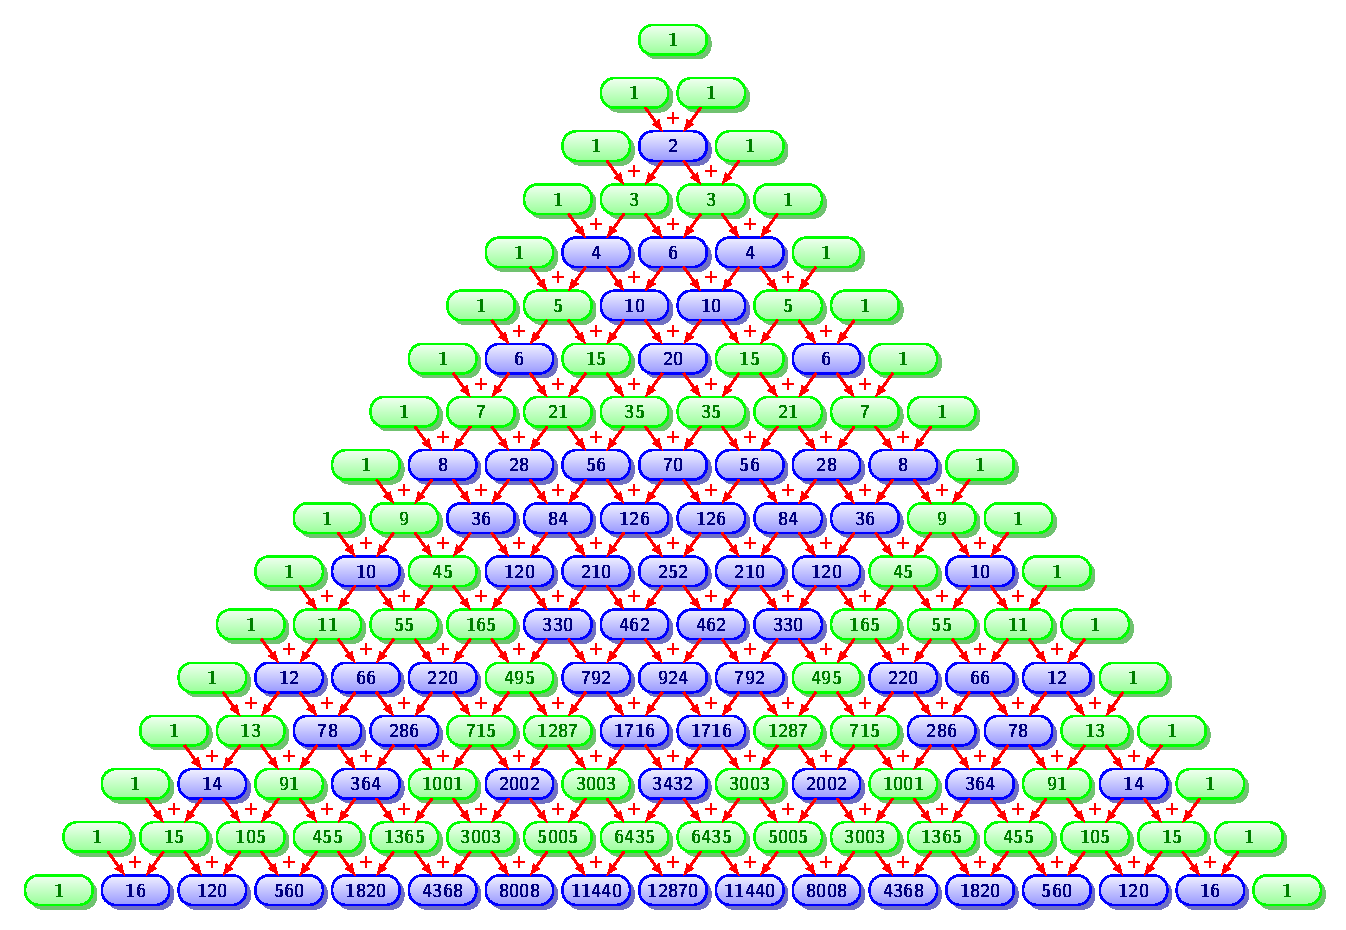
\includegraphics[width=1\textwidth,height=0.6\textheight]{pascals-triangle-and-sierpinski-triangle}\caption{Pascal and Sierpinski Triangle} \label{pascal}
\end{figure}
{}\index{Pascal triangle}
	    \paragraph{Factorials}
If $n$ is a natural number, then $n!$ is defined as
      \begin{equation}
    \boxed{n! = n(n-1)(n -2)(n -3) \cdots (3)(2)(1)} 
      \end{equation}
Two properties of factorials\index{factorial} include
\begin{property}
    \textbf{Identity} By definition, $0! = 1$.
\end{property}
\begin{property}
    \textbf{Equivalence} If n is a natural number, then $n(n -1)! = n!$.
\end{property}
A couple examples should suffice:

   \begin{equation}
\begin{split}
    3! = 3 * 2 * 1 = 6 \\
6! = 6*5*4*3*2*1 = 720  \\
3(3-1)! = 3*\textcolor{red}{2} = 6 \textcolor{blue}{= 3!} \\
\end{split}
   \end{equation}

   \subsection{Binomial Theorem}
If $n$ is any positive number, then
	 \begin{equation*}
   \colorbox{Honeydew2}{(a+b)$^n$ =}
	 \end{equation*}
      \begin{equation}
	    \begin{split}
       \color{Blue4}a^n + \frac{n!}{1!(n-1)!)}a^{n-1}b + \frac{n!}{2!(n-2)!}a^{n-2}b^2 + \\ 
\color{Blue4}\frac{n!}{3!(n-3)!)}a^{n-3}b^3 + \cdots + b^n
	    \end{split}
	  \end{equation}

There is a more compact way to write the theorem using summation notation. I give the compact version here but lead up to it in the next section; see equation \ref{bin-summation}.
\begin{equation*}
   \textcolor{Brown4}{\sum_{r=0}^{n}\frac{n!}{r!(n - r!)}a^{n-r}b^r}
\end{equation*}


      \section{Summation}\index{$\sigma$}
A shorthand way to indicate the sum of the first $n$ terms, or the $n$th partial term, of a sequence\index{sequence}. Notice that because summation\index{summation} shows which $n$th terms are to be used the arbitrariness of subsequences noted above no longer applies. That is, in $\sum_n^m$ the $n$ value tells us where to start the numerical sequence\index{numerical sequence} and the $m$ term tells us how far to go in the sequence.  
\begin{align}
    \sum_{n=1}^{3}(2n^2 + 1) & \nonumber \\
&= [2(\textcolor{red}{1})^2 + 1] + [2(\textcolor{red}{2})^2 + 1] + [2(\textcolor{red}{3})^2 + 1] \nonumber \\
&= 3 + 9 + 19\nonumber \\
&= 31
\end{align}
In this example there is no arbitrariness about where to begin the subsequence and how far to go in the sequence; nor about the systematicity of the interval partitions -- at least not in this example (i.e., by numerical values of 1). The bottom domain\index{domain} tells us where to start (e.g., $n =1$: start at 1), and the upper domain tells us how far to go (e.g., numerical value 3). One more example should suffice; notice that the upper domain is 5 and the lower one is 3. This does not mean start at 3 and continue 5 sequence steps, such as $a_5$. Instead, it means start at 3 and work our way up to 5, which is three sequential steps $a_3$; or more acurately $a_3 \to a_4 \to a_5$.
\begin{align}
     \sum_{n=3}^{5}(3n + 2) & \\
&= [3(\textcolor{red}{3})+2] + [3(\textcolor{red}{4})+2] + [3(\textcolor{red}{5})+2] \nonumber \\
&= 11 + 14 + 7 \nonumber \\
&= 42 \nonumber
\end{align}

	 \subsection{Three Basic Properties of Summation}\index{summation}
\begin{property}\textbf{Summation of a constant.}\index{summation of constant}
    The summation of constant (c) as the value k runs from 1 to n is n times the constant.  
\end{property}
   \begin{equation}
    \boxed{\text{If $c$ is constant, then} \sum_{k=1}^n c = nc.}
   \end{equation}
For example,
      \begin{equation}
	  \boxed{\sum_{k=1}^5 13 = 13_1 + 13_2 +13_3 +13_4 +13_5 = 5(13) = 65}
      \end{equation}
\begin{proof}
    Because $c$ is a constant, each term $c$ is constant for each value $k$ as $k$ runs from 1 to $n$.
\[
    \sum_{k=1}^nc = \overbrace{c +c +c +c +c + \cdots +c}^\text{\textcolor{red}{$n$ number of $c_k$}} = nc
\]
\end{proof}


\begin{property}\textbf{Summation of a product.}\index{summation of product}
    A constant factor can be brought outside a summation sign.
\end{property}
   \begin{equation}
       \boxed{\text{If $c$ is constant, then} \sum_{k=1}^n cf(k) = c\sum_{k=1}^n f(k).}
   \end{equation}
For example, 
      \begin{equation*}
          \boxed{\text{Show that} \\ \sum_{k=1}^3\textcolor{red}{5}k^2 = \textcolor{red}{5}\sum_{k=1}^3k^2}
      \end{equation*}
	 \begin{align}
\sum_{k=1}^3\textcolor{red}{5}k^2 &= \textcolor{red}{5}(1)^2 + \textcolor{red}{5}(2)^2 + \textcolor{red}{5}(3)^2 &  \textcolor{red}{5}\sum_{k=1}^3k^2 &= \textcolor{red}{5}[(1)^2 + (2)^2 + (3)^2]\nonumber \\
&= \textcolor{red}{5} + 20 + 45       &            &= \textcolor{red}{5}[1 + 4 + 9]\nonumber \\
&= \textbf{70}				       & 	    &= \textcolor{red}{5}(14) = \textbf{70}
\end{align}
      \begin{proof}
	 \begin{align*}
  \sum_{k=1}^ncf(k) &= cf(1) + cf(2) + cf(3) + \cdots + cf(n)\\
&= c[f(1) + f(2) + f(3) + \cdots + f(n)] \; \; \text{\textcolor{magenta}{(Factor out $c$)}}\\
&= c\sum_{k=1}^nf(k) 
	 \end{align*}
      \end{proof}


\begin{property}\textbf{Summation of a sum.}\index{summation of sum}
    The summation of a sum is equal to the sum of the summations.
\end{property}
   \begin{equation}
       \boxed{\sum_{k=1}^n [f(k) + g(k)] = \sum_{k=1}^n f(k) + \sum_{k=1}^n g(k).}
   \end{equation}
For example, 
\begin{equation*}
    \boxed{\text{Show that} \sum_{k=1}^3\textcolor{red}{(k + k^2)} = \sum_{k=1}^3\textcolor{red}{k \ +} \sum_{k=1}^3\textcolor{red}{k^2}}
\end{equation*}
\begin{align}
    \sum_{k=1}^3\textcolor{red}{(k + k^2)} &= (1 + 1^2) + (2 +2^2) +(3 + 2^2)\nonumber \\
&= 2 + 6 + 12 = \textbf{20} \nonumber \\
\sum_{k=1}^3\textcolor{red}{k \ +} \sum_{k=1}^3\textcolor{red}{k^2} &= (1 + 2 +3) + (1^2 + 2^2 + 3^2) \nonumber \\
&= 6 + 14 = \textbf{20} 
\end{align}
\begin{proof}
    \begin{align*}
       \sum_{k=1}^n [f(k) + g(k)]& \\
&= [f(1) + g(1)] +[f(2) + g(2)] + \cdots + [f(n) + g(n)]\\
&= [f(1) + f(2) + \cdots + f(n)] + [g(1) + g(2) + \cdots + g(n)]\\
&= \sum_{k=1}^n f(k) + \sum_{k=1}^n g(k)
    \end{align*}
\end{proof}


	 \subsection{Binomial theorem as summation}\index{binomial summation}
\begin{equation}
   \sum_{r=0}^{n}\frac{n!}{r!(n - r!)}a^{n-r}b^r
\end{equation}\label{bin-summation}

\section{Induction}
A general definition for mathematical induction is based on the successor function. This is a now classic method made standard by Giuseppe Peano around the beginning of the 20th century; in which the arithmetic of cardinal numbers of axiomatized. Typically, we define a primitive and some kind of binary combinatoric operation (i.e., addition and/or multiplication), and then simply iterate the primtive and combining operation.\footnote{It is hard to overemphasize the importance of the use of induction to contemporary formalization.}

A very common model for successor functions and induction is the domain of the whole numbers. The primitive is zero and the combinatory operation is addition (or multiplication). To this model we apply the axioms of Peano.
Begin with three primitive (undefined and unmotivated) terms: \textbf{number}, \textbf{zero}, and \textbf{immediate successor of}. The following axioms can be given:

\newtheorem{peanoaxiom}{Peano Axiom}
\begin{peanoaxiom}
    Zero is a number
\end{peanoaxiom}
\begin{peanoaxiom}
    The immediate successor of a number is a number.
\end{peanoaxiom}
\begin{peanoaxiom}
    Zero is not the immediate successor of a number.
\end{peanoaxiom}
\begin{peanoaxiom}
    No two numbers have the same immediate successor.
\end{peanoaxiom}
\begin{peanoaxiom}\label{induction}
    Any property belonging to zero, and also to the immediate successor for every number that has the property, belongs to all numbers.
\end{peanoaxiom}

The last axiom is referred to as the \textsc{Principle of Mathematical Induction}; this reflects that understanding that the last `axiom' is not technically an axiom; it may also be a called an \textsc{Induction Axiom Scheme}. Peano's axioms can be formally represented as follows.

\subsection{A Formalized Induction Scheme for Peano's Axioms} 

\begin{align}
    \text{Peano Axiom 3} \ \quad \neg0 &= sx \label{rpaxiom3}\\
   \text{Peano Axiom 4} \ \quad sx &= sy \rightarrow x = y \label{rpaxiom4}
\end{align}
\ref{rpaxiom3} says that the \textcolor{teal}{negation of zero is a number with a successor}, or conversely, \textcolor{olive}{if a number has no successor, then it must be zero}, or that \textcolor{blue}{zero is not the successor of any number}. \ref{rpaxiom4} says that \textcolor{teal}{if the successor of x equals the successor of y, then x equals y}, or in other words, \textcolor{blue}{given any number, its predecessor is unique}. Now we can provide representations for axioms of the binary operations addition, $+$, and multiplication, $*$, 
\begin{align}
    x + 0 &= x\label{add0}\\
   x + sy &= s(x + y)\label{adds}\\
   x * 0 &= 0\label{times0}\\
   x * sy &= x * y + x\label{timess}
\end{align}
\ref{add0} is the identity of addition (any number $x$ added to zero sums to that number $x$); \ref{adds} says that any number $x$ plus the successor of $y$ is equivalent to the successor of $x + y$; \ref{times0} is straightforward, and \ref{timess} says that any number $x$ times the sucessor of the number $y$ is equivalent to $x * y$ plus the number $x$.

To the representations in \ref{rpaxiom3}--\ref{timess} we can add the following instance of the induction scheme, or principle of mathematical induction, from \ref{induction}.

Given any formula with a free variable $x$, $P(x)$, we can get the following instance of induction
\begin{equation}
    (P(0) \& \forall x(P(x)) \rightarrow P(s(x))) \longrightarrow \forall xP(x)
\end{equation}
What this says is that \textcolor{teal}{for the property $P$ that belongs to $0$, and for all $x$ with that property, then the successor of $x$, $sx$, also has that property, $P(s(x))$; If the latter is the case, then this will hold for all $x$}.

\subsubsection{Writing numerals inductively}
The common way of writing the Arabic numerals in the set of whole numbers, ${0, 1, 2, 3, 4, \ldots, n}$, implies the inductive principle and is an efficient way to compact the information in that principle. A more explicit way to write the set whole numbers is the following (I also show the correlation with Arabic numerals):
\begin{equation}
    \begin{split}
        0 = 0\\
	 0s = 1\\
	 0ss = 2\\
	 0sss = 3
\end{split}
\end{equation}	

Addition of $2 + 2 = 4$ looks like this (the second representation is in Polish notation and is equivalent with the first):
\begin{align*} 
s(s(0)) + s(s(0)) &= s(s(s(s(0)))).\\
&\text{or,}\\
 +(s(s(0)), \ s(s(0)) &= s(s(s(s(0))))).
\end{align*}


\paragraph{Division in a formalized induction scheme}
Induction is defined for binary combinatoric operations multiplication and addition. But we can also define division as (assume the definitions \ref{add0}--\ref{timess}):
\begin{equation}
    \exists z(x *z = y)
\end{equation}

\section{Induction and Sequences}
Another way to get at induction is through arithmetical sequences (a-sequences); see section \ref{a-seq}. As a transition I show an alternate way to write the addition of numerals as an inductive scheme:
\begin{align}
    A_0^3 &= 3 + 0 = 3 \nonumber \\
   A_1^3 &= 3 + 1 = 4 \nonumber \\
   A_2^3 &= 3 + 2 = 5
\end{align}
Another way to write this would be as
\begin{align*}
    A_0^3 &= 3 + 0 = 3  \\
   \textcolor{blue}{A_1^3} &= \textcolor{blue}{(3 + 1) = (3 + 0s) = (3 + 0)s = 4} \\
   \textcolor{teal}{A_2^3} &= \textcolor{teal}{(3 + 2) = (3 + 0ss) = (3 + 0s)s = ((3 + 0)s)s = 5}
\end{align*}
The first line needs no explanation. The second line says that \textcolor{blue}{three plus one is equal to three plus the successor of zero, which itself is equal to the successor of three plus zero}, which is 4. The third line says that \textcolor{teal}{three plus two is equal to  three plus the successor of the successor of 0, which itself is equal to the successor of three plus the successor of zero, which is itself equal to the successor of the successor of three plus 0}, which is 5. If ever there was a motivation for using Arabic numerals, this would be one: Arabic numerals implicitly provide the inductive information contained in their respective numerical values. In fact, the information is so implicit and assumed, that most college educated people are unable to provide a proof of why simple addition works. This is because we don't need to, the additive operation already contains the information needed for proof of the mathematical inductive principle. 

A still yet more explicit way of writing this is
\begin{align*}
    A_0^{0sss} &= (0sss + 0) = (0sss) = 3 \\
   \textcolor{blue}{A_{0s}^{0sss}} &= \textcolor{blue}{(0sss + 0s) = (0ssss) = 4} \\
   \textcolor{teal}{A_{0ss}^{0sss}} &= \textcolor{teal}{0sss + 0ss = (0sssss) = 5}
\end{align*}
What this suggests is that we can think of numerals defined through an induction scheme, or induction principle, as similar to a-sequences. That is, adding the sequence of successors defines the cardinality of the numerical value. This is an interesting point of relation between induction and a-sequences: a numerical value itself, say $4$, can be derived through adding all the successors together.\footnote{Multiplication can be shown in the same way, except that instead of counting successors by a value of 1, we count successors by the value of the multiplicand. For example, if the mulitplicand is 3, then we count successive values by increments of 3: $3 * 2$ is equivalent to counting two times by increments of 3, $= (3, 6) = (3 + 3) = 6$. Another example, $5 * 4$ is equivalent to counting four times by increments of 5, $= (5, 10, 15, 20) = (5 + 5+ 5 + 5) = 20$; So on and so on.} 


 




















 


%===========Comment out for Book=========
\end{document}
%====================

%===================
%===========Comment out for Book==================
\documentclass{book} \usepackage{mathpackages} \begin{document} 
%====================================

\chapter{Probability}
The basic expression for showing a relationship for the probability $P$ between two (or more) events is
\begin{equation}
    P(Event) = \frac{\text{The number of outcomes involving E}}{\text{The total number of possible outcomes}}
\end{equation}
\begin{law}\textsc{Addition Law for Probabilities}
    \[P(E \ or \ F) = P(E) + P(F) - P(E  *  F)\]
\end{law}
 


%===========Comment out for Book=========
 \end{document}
%====================



%=====================
\bibliography{mathrefs}
%===============uncomment this when I want to print index======
\printindex
%===========


\end{document}
